
\section{Implementation}

\subsection{Project Structure}

One of the 


\begin{figure}[t!]
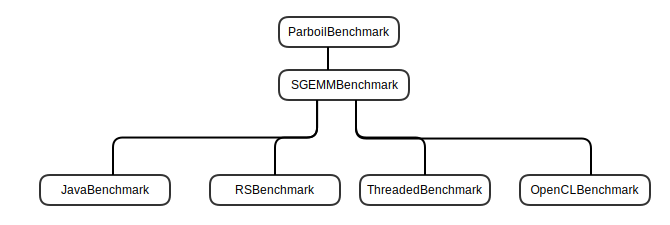
\includegraphics[scale=0.43, angle=90]{class_arch.pdf}
\caption{Project Class Structure.}
\label{fig:projclass}
\centering
\end{figure}


\subsection{Timer}



\subsection{Output}


\begin{figure}[t!]
\begin{verbatim}
struct {
	string Type,
	string Hardware,
	string Benchmark,
	string Implementation,
	string Category,
	string Message,
	long StartTime,
	long EndTime,
	long ElapsedTime,
	string Data,
	string Date,
}
\end{verbatim}
\caption{Database Columns.}
\label{fig:database}
\centering
\end{figure}

Unlike Parboil, which outputs the times to {\tt stdout}, we output our data into a SQLite database.
This affords us a few things.
First, since data is outputed in the specified columns, we do not have to reparse the output data.
Second, timing information can be shared easily by copying the database.
Finally, we can store more than just timing information.

